\documentclass[12pt, letterpaper]{article}

\usepackage{graphicx}
\usepackage{parskip} % Disabling paragraph index as it does not fit maths
\usepackage{amssymb} % Used to show sets of sumbers, like the real numbers
\usepackage{amsmath} % Used for picewise functiong
\usepackage{hyperref} % Usable menu and references

\graphicspath{{images}}

\title{Elementary Number Theory}
\author{Arkadiusz Naks}
\date{2023}

\begin{document}

\begin{titlepage}
  \begin{center}
    \makeatletter
    \vspace*{1cm}
    \Huge
    \textbf{\@title}

    \vspace{0.5cm}
    \Large
    Lecture notes from Elementary Number Theory module at Durham University

    \vspace{1.5cm}

    \textbf{\@author}

    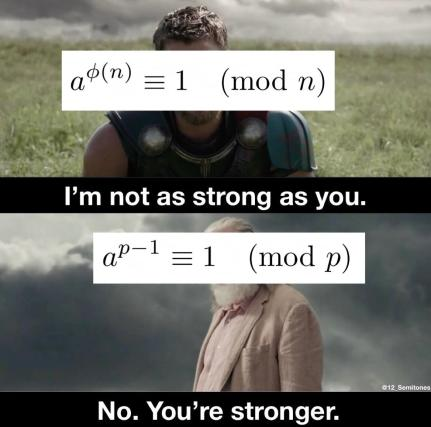
\includegraphics[scale=0.55]{ent.png}
    \vfill

    \vspace{0.8cm}

    \small
    Based on my understanding of lectures and notes of Prof Alexander Sacha Mangerel,
    \@date{}
  \end{center}
\end{titlepage}

\tableofcontents
\newpage

\begin{section}{Important Definisions}

  A place for short and important definisions \\

  \textsc{Definision} (Divisibility) \textit{For \(a, b \in \mathbb{Z}\) a
    \textbf{divides} b, denoted \(a | b\) if \(\exists d \in \mathbb{Z}\) s.t.
    \(b = ad\). Otherwise \(a \nmid b\).}

  \textsc{Definision} (Diophantine Equation) \textit{An equation where we seek
    integer or rational solution; very important in number theory}

\end{section}

\begin{section}{Some Basics}

  \begin{subsection}{Sets}

    Firstly the natrual numbers \[\mathbb{N} = \{ 1, 2, 3, \dots \}\]
    Then \[\mathbb{N}_{0} = \{ 0, 1, 2, \dots \} = \mathbb{N} \cup \{ 0 \}\]
    Some axioms about \(\mathbb{N}_{0}\)
    \begin{itemize}
      \item \(0 \in \mathbb{N}_{0}\)
      \item \(\forall a \in \mathbb{N}_{0} S(a) \neq 0\)
      \item \(\forall a, b \mathbb{N}_{0}\) if \(S(a) = S(b) \to a = b\)
      \item If \(X \subset \mathbb{N}_{0}\) s.t.
            \begin{itemize}
              \item \(0 \in X\)
              \item \(a \in X \to S(a) \in X\)
            \end{itemize}
            Then \(X = \mathbb{N}_{0}\)
    \end{itemize}

    \(S(a)\) is another way of saying \(a + 1\) but addition is not yet defined.

    \(\mathbb{Z} = \{ 0, \pm 1, \pm 2, \dots \}\) \\
    \(\mathbb{Q} = \{ \frac{a}{b} | a, b \in \mathbb{Z}, b \neq 0 \}\)

    \textbf{Well Ordered Principle}. Let \(S \subset \mathbb{N}_{0}, S \neq \emptyset\)
    then S has a smallest element.

  \end{subsection}

  \begin{subsection}{Divisiblity}

    Some propersies of the definision above
    \begin{itemize}
      \item \(a | 0\)
      \item \(0 \nmid b\) if \(b \neq 0\)
      \item \(1 | a\) and \(a | a\)
      \item \(a | b \to a | bc\)
      \item \(a | b\) and \(b | c \to a | c\)
      \item \(a | b\) and \(a | c \to a | (bx + cy)\) for any x, y
      \item \(a | b\) and \(b | a \to a = \pm b\)
      \item If \(a, b > 0\) and \(a | b \to a \leq b\)
      \item \(a | b \to ac | bc\)
    \end{itemize}

    \textbf{Long division}. For \(a \in \mathbb{Z}\) and \(b \in \mathbb{N} \; \exists q, r \in \mathbb{Z}\)
    s.t. \(a = qb + r\) and \(0 \leq r < b\). \\
    \emph{If \(a | b\) then \(r = 0\)} \\

    \textbf{Greatest common divisior} is defined to be \(d \in \mathbb{Z}\) s.t.
    \(d | a\) and \(d | b\) and d is \textbf{maximal}. This is denoted as \(\gcd(a, b) = d\).
    If \(\gcd(a, b) = 1\) a and b are called \textbf{coprime}. \\
    \emph{If \(a = b = 0\) then \(\gcd(a, b)\) does not exist} \\
    Properties of gcd
    \begin{itemize}
      \item \(\gcd(a, b) = \gcd(b, a) = \gcd(-a, b)\)
      \item \(a > 0 \to \gcd(a, b) = a\)
      \item \(a, b < 0 \to \gcd(a, b) \leq \min\{ a, b \}\)
      \item For \(a, b \exists q\) s.t. \(\gcd(a, b) = \gcd(a, b - aq)\)
    \end{itemize}

    \emph{\(\gcd(a, b) = ax + by | x, y \in \mathbb{Z}\)}

  \end{subsection}

\end{section}

\begin{section}{Prime Numbers}

  \begin{subsection}{Basics}

    \(n \in \mathbb{N}\) is called \textbf{prime} if \(n > 1\) and if
    \(d | n \to d = n \; or \; d = 1\). Otherwise \(n > 1\) is called \textbf{composite}.
    There are infinitely many primes and there are infinitely many primes of the
    form \(4n - 1\). More generaly if a, b are \textbf{coprime} there are infinitely
    many primes of \(an + b\) form. \\
    \emph{0 and 1 are neither \textbf{composite} or \textbf{prime}} \\
    Euclid's Lemma: p is prime iff \(\forall a, b \in \mathbb{Z}\) we have
    \(p | ab \to p | a \; or \; p | b\).

    For \(n \in \mathbb{N}, \; n > 1\) there exists distinct series of
    \(p_{1}, \dots, p_{r}\) and \(e_{1}, \dots, e_{r} \in \mathbb{N}\) s.t.
    \[n = p_{1}^{e_{1}} p_{2}^{e_{2}} \dots p_{r}^{e_{r}}\]

  \end{subsection}

  \begin{subsection}{Open Problems about primes}

    \begin{itemize}
      \item Are there infinitely many primes of the form \(n^{2} + 1\) (probs true)
      \item Are there infinitely many twin prime \\
            primes p s.t. \(p + 2\) is also prime
      \item Is every even number \(n > 2\) the sum of two primes //
            Goldblach's conjecture
    \end{itemize}

  \end{subsection}

  \begin{subsection}{Pythagorean Theorem}
    A \textbf{pythagorean triple} \((x, y, z) \in \mathbb{N}^{3}\) is a solution
    of the equasion \(x^{2} + y^{2} = z^{2}\). It is called \textbf{primitive}
    if \(\gcd(x, y, z) = 1\). If \((x, y, z)\) is a pythagorean triple then
    \((kx, ky, kz)\) is a pythagorean triple \(\forall k \in \mathbb{N}\).

    For a triple to be primitive \textbf{precisely one} of x and y is \textbf{even}
    and z is \textbf{odd}. Defining \[u := \frac{z + y}{2} , \;\; v := \frac{z - y}{2}\]
    and therefor \[\frac{x}{2}^{2} = uv.\]
    If u, v are coprime they are squares. \\
    We can also define \[s^{2} = u , \;\; t^{2} = v\]
    meaning \(1 \leq t < s\) and \[z = s^{2} + t^{2}, \;\; y = s^{2} - y^{2}, \;\; x = 2st.\]

    All \textbf{primitive} Pythagorean triples \((x, y, z)\) with \(2 | x\) are given by
    \[\begin{cases}
        x = 2st \\
        y = s^{2} - t^{2} \\
        z = s^{2} + t^{2}
      \end{cases}
    \]
    for \(s > t \geq 1\) such that \(\gcd(s, t) = 1\) and \(s \not\equiv t \pmod{2}\)

    A more general equasion is \(x^{n} + y^{n} = z^{n}, \; n > 2\). In this case
    there are \textbf{no} solutions in \textbf{natural numbers}.
    \(x^{2} + y^{4} = z^{2}\) also has no solutions in natural numbers.

  \end{subsection}

\end{section}

\begin{section}{Modular Arithmetics}

  \begin{subsection}{Basics}

    For \(a, b, n \in \mathbb{Z}\) if \(n | (a - b)\) is equivalent to
    \(a \equiv b \pmod{n}\). For \(n \in \mathbb{N}\) if \(a \equiv a' \pmod{n}\)
    and \(b \equiv b' \pmod{n}\) then
    \begin{itemize}
      \item \(a + b \equiv a' + b' \pmod{n}\)
      \item \(ab \equiv a'b' \pmod{n}\)
    \end{itemize}

    \emph{In general we cannot divide both sides of a congurance}

    For \(a, b, c, n \in \mathbb{N}\) s.t. \(\gcd(c, n) = 1\) then
    \(ac \equiv bc \pmod{n}\) \(\iff a \equiv b \pmod{n}\).
    As said above this is always true only if c and n are coprime.

    \textbf{Complete set of residues} mod n is a subset \(R \subset Z\), size n,
    whose remainders are all different.

  \end{subsection}

  \begin{subsection}{Congruences}

    \begin{subsubsection}{Linear Congruences}

      For known \(a, b, n \in \mathbb{Z}\) and unknown \(x \in \mathbb{Z}\)
      a \textbf{linear congurance} is defined to be \(ax \equiv b \pmod{n}\). If this
      has a solution, it is unique up to multiples of n. The solution exists iff
      \(\gcd(a, n) | b\).

      To solve a linear congurance we assume \(\gcd(a, n) = 1\) then
      \begin{itemize}
        \item Use the Euclidian Algorithm to find \(u, v \in \mathbb{Z}\) s.t.
              \(1 = au + nv\)
        \item \(au \equiv 1 \pmod{n}\) \(\to a(ub) \equiv b \pmod{n}\).
              So \(x = ub\) is the basic solution. \(x + kn \; \forall k \in \mathbb{N}\)
              is also a solution.
      \end{itemize}

    \end{subsubsection}

    \begin{subsubsection}{Chinese Remainder Theorem}

      For \(m, n \in \mathbb{N}\) coprime and \(a, b \in \mathbb{Z}\) then
      \(\exists x \in \mathbb{Z}\) s.t. \[x \equiv a \pmod{m}\] \[x \equiv b \pmod{n}\]
      And any two solutions are congured mod(mn). It is also unique (up to multiple of mn).
      The solution is \(x = asn + brm\) where \(s, r\) are found through Euclidian
      Algorithm, \(1 = rm + sn\).

    \end{subsubsection}

  \end{subsection}

  \begin{subsection}{Euler Function}

    Euler func \(\varphi: \mathbb{N} \to \mathbb{N}\) is defined as
    \(\varphi(n) = \#\{ r \in \mathbb{N} | \; r \leq n, \; \gcd(r, n) = 1 \}\).
    In words it is the number of coprime to n and smaller than n.

    For any prime p, \(\varphi(p) = p - 1\) and \(\varphi(p^{n}) = p^{n}(1 - \frac{1}{p})\). \\
    For any \(m, n \in \mathbb{N}\) s.t. \(\gcd(n, m) = 1\) we have
    \(\varphi(mn) = \varphi(m) \varphi(n)\).

    Formulation of \(\varphi(n)\) for \(n \in \mathbb{N}\) then
    \[\varphi(n) = n \Pi^{r}_{i = 1}(1 - \frac{1}{p_{i}})\] where
    \(n = \Pi^{r}_{i = 1} p_{i}^{a_{i}}\) is \textbf{prime factorisation} of n.
    As it can be seen the Euler function is not dependent on the powers \(a_{i}\).

    Another properti of the Euler function is that \(\sum_{d | n} \varphi(d) = n\),
    meanign the Euler functions of divisors of n add up to n.

    For \(n \in \mathbb{N}\) and \(a \in \mathbb{Z}\) s.t. \(\gcd(a, n) = 1\) we
    have \[a^{\varphi(n)} \equiv 1 \pmod{n},\] meaing any number to the power of
    Euler function of n is one mod n if it shares no common factors with n.
    This means for prime p and \(a \in \mathbb{Z}\) s.t. \(p \nmid a\) then
    \(a^{p - 1} \equiv 1 \pmod{p}\).

  \end{subsection}

  \begin{subsection}{Primitive Roots}

    Very many propositions, theorems and lemmas. They can be veryy useful in
    theory s.t. Euler's criterion and practical s.t. Diffie-Hellman key exchange
    cryptosystem.

    For \(n \in \mathbb{N} \; and \; a \in \mathbb{Z}\) coprime
    \textbf{multiplicative order} of a mod n, denoted \(ord_{n}(a)\), is the
    smallest \(d \in \mathbb{N}\) s.t. \[a^{d} \equiv 1 \pmod{n},\] and
    \(ord_{n}(a) \leq \varphi(n)\). \\
    Any d s.t. \(a^{d} \equiv 1 \pmod{n} \to ord_{n} | d\). This also means
    \(ord_{n}(a) | \varphi(n)\).

    For \(n \in \mathbb{N}\) coprime to \(a \in \mathbb{Z}\) a is called a
    \textbf{primitive root mod n} if \(ord_{n}(a) = \varphi(n)\).

    For a prime p, any \(f(x) \neq 0\) of degree n with integer coefficients has
    at most n roots mod p, meaning there are at most n xs s.t. \(f(x) \equiv 0 \pmod{p}\).

    For \(d | (p - 1)\), the congurance \(x^{d} - 1 \equiv 0 \pmod{p}\) has
    exacly d solutions.

    For a prime p, there exist exacly \(\varphi(p - 1)\) primitive roots mod p.

    If g is a primitive root mod p then any \(a \in \mathbb{Z}\) coprime to p
    can be written as \(a \equiv g^{r} \pmod{p}\) for some \(r \in \mathbb{N}\).
    This means a primitive root is precisely a generator of the group \((\mathbb{Z} / p)^{x}\)

    Primitive roots mod n exist iff n is \(2, 4, p^{k}, 2p^{k}\) for any p prime
    and \(p \neq 2\) and any \(k \in \mathbb{N}\).

  \end{subsection}

  \begin{subsection}{Quadratic Residues}

    This is about solving \(x^{2} \equiv a \pmod{p}\) for prime \(p \neq 2\).

    For p prime and \(a \in \mathbb{Z}\) coprime to p, then a is \textbf{quadratic
      residue (QR)} mod p if \(\exists x \in \mathbb{Z}\) s.t.
    \(x^{2} \equiv a \pmod{p}\). Otherwise a is \textbf{quadratic non-residue NR}.
    For an odd p, there are exacly \(\frac{p - 1}{2}\) quadratic residues.

    Rules for products of QRs and NRs:
    \begin{itemize}
      \item \(QR \times QR = QR\)
      \item \(QR \times NR = NR\)
      \item \(NR \times NR = QR\)
    \end{itemize}
    As seen above, product of residues follow same rulles as
    odd and even addition.

    \begin{subsubsection}{Legendre Symbol}

      To calculate  whenether something is QR or NR, Legendre symbol is used.
      This is defined as
      \[(\frac{a}{p}) =
        \begin{cases}
          1 & a = QR \\
          -1 & a = NR \\
          0 & p | a
        \end{cases}
      \]

      Some properies of Legendre
      \begin{itemize}
        \item \((\frac{ab}{p}) = (\frac{a}{p})(\frac{b}{p})\)
        \item \((\frac{a}{p}) = (\frac{b}{p})\) if \(a \equiv b \pmod{p}\)
        \item \((\frac{0}{p}) = 0\)
        \item \((\frac{1}{p}) = 1\)
      \end{itemize}

      For p and \(a \in \mathbb{Z}\) coprime we have
      \(a^{\frac{p - 1}{2}} \equiv (\frac{a}{p}) \pmod{p}\).

      A procedure for calculating Legendre symbol of \((\frac{a}{p})\)
      \begin{enumerate}
        \item Long division on a, p with remainder r then \((\frac{a}{p}) = (\frac{r}{p})\)
        \item \((\frac{r}{p}) = (\frac{q_{i}}{p})\) for \(q_{i}\) are all prime factors of r
        \item Calculate each factor product same procedure
      \end{enumerate}

      Some rules:
      \begin{itemize}
        \item \((\frac{2}{p}) = (-1)^{\frac{p^{2} - 1}{8}}\)
        \item \((\frac{a}{p}) = (\frac{p}{a})(-1)^{\frac{p - 1}{2} \frac{a - 1}{2}}\)
      \end{itemize}
      
    \end{subsubsection}

  \end{subsection}

  \begin{subsection}{Sum of Two Squares}

    If both m and n are  sums of two squares then mn is also. \\
    \emph{Odd prime p is only sum of two squares if \(p \equiv 1 \pmod{4}\)}

  \end{subsection}

\end{section}

\begin{section}{Continued Fractions}

  \begin{subsection}{Basics}

    All real numbers can be represented by a continued fraction. This can be
    used to solve certain problems, like for example Pell equations
    \(x^{2} - dy^{2} = \pm 1, \; d \in \mathbb{N}, \; x, y \in \mathbb{Z}\).

    Continues fraction (CF) is denoted as \[[a_{0}; a_{1}, a_{2}, \dots , a_{n}]\]
    which means:
    \[a_{0} + \cfrac{1}{a_{1} + \cfrac{1}{a_{2} + \cfrac{1}{\ddots + \cfrac{1}{a_{n}}
          }}}\]
    where all \(a_{i} \in \mathbb{R}\). If \(a_{0} \in \mathbb{Z}\) and
    \(a_{i} \in \mathbb{N} \;|\; i < 0\) then the fraction is called simple.

    \emph{Any rational number can be expressed as a \textbf{finite simple continued fraction}}

  \end{subsection}

  \begin{subsection}{Convergant}

    k-th convergent of \([a_{0}; a_{1}, \dots , a_{n}]\) for \(k \leq n\) is
    \(C_{k} = [a_{0}, a_{1}, \dots , a_{k}]\).

    \[
      \begin{bmatrix}
        p_{k} & p_{k - 1} \\
        q_{k} & q_{k - 1}
      \end{bmatrix} =
      \begin{bmatrix}
        a_{0} & 1 \\
        1 & 0
      \end{bmatrix}
      \begin{bmatrix}
        a_{1} & 1 \\
        1 & 0
      \end{bmatrix}
      \dots
      \begin{bmatrix}
        a_{k} & 1 \\
        1 & 0
      \end{bmatrix}
    \]

    This ps and qs can be used to calculate the convergent, using
    \(C_{n} = \frac{p_{n}}{q_{n}}\). \\
    To calculate the ps and qs we use the formula above to deduce
    \[
      \begin{bmatrix}
        p_{1} & p_{0} \\
        q_{1} & q_{0}
      \end{bmatrix} =
      \begin{bmatrix}
        a_{0}a_{1} + 1 & a_{0} \\
        a_{1} & 1
      \end{bmatrix}
    \]
    and then for \(k > 1\)
    \[p_{k} = a_{k}p_{k - 1} + p_{k - 2}\]\[q_{k} = a_{k}q_{k - 1} + q_{k - 2}\]

    \(p_{k}q_{k - 1} - q_{k}p_{k - 1} = (-1)^{k + 1}\) for all \(k \geq 1\).
    This means \(\gcd(p_{k}, q_{k}) = 1\) and all even \(C_{i}\) are below the target
    value and all odds are above the target value.

    A convergance error boundary can be specified as
    \[|\alpha - \frac{p_{k}}{q_{k}}| \leq \frac{1}{q_{k}q_{k + 1}}\] where
    \(\alpha\) is the actuall number.

  \end{subsection}

  \begin{subsection}{Infinite}

    An infinte CF is a is the limit of the convergents \(C_{n}\). The limit
    always exists. \\
    An infinte CF is called periodic if it is constructed of a repeating
    sequence, or \(a_{i} = a_{j}\) if \(i \equiv j \pmod{n}\) with n the period.
    A CF can only become periodic from any \(a_{i}\). \\
    For \(d \in \mathbb{N}\) and d not square the infinite CF of \(\sqrt{d}\)
    is periodic after \(a_{0}\).

  \end{subsection}

  \newpage

  \begin{subsection}{Pell's Equation}

    As mentioned above, Pell's equation is \(x^{2} - dy^{2} = 1\) where
    \(d \in \mathbb{N}\) and d not a square and we seek solution \(x, y \in  \mathbb{N}\).
    While solving this the trivial result \((x, y) = (1, 0)\) is usually discounted.
    Negative Pell equation is \(x^{2} - dy^{2} = -1\).

    The CF of \(\sqrt{d}\) can be used to solve the Pell equations if solutions
    exist. For n begin the period of CF of d \[p^{2}_{kn - 1} - dq^{2}_{kn - 1} = (-1)^{kn}.\]
    Where \(k > 0\) is any integer.
    This can be summerised into the following rules:
    \begin{itemize}
      \item If n even
            \begin{itemize}
              \item \((x, y) = (p_{kn - 1}, q_{kn - 1})\) for positive Pell
              \item No anwser for negative Pell
            \end{itemize}
      \item if n odd
            \begin{itemize}
              \item \((x, y) = (p_{2kn - 1}, q_{2kn - 1})\) for positive Pell
              \item \((x, y) = (p_{(2k - 1)n - 1}, q_{(2k - 1)n - 1})\) for negative Pell
            \end{itemize}
    \end{itemize}

    \emph{Importantly this gives an expression for all solutions}

  \end{subsection}

\end{section}

\end{document}
